\chapter{绪论}
\label{chap:chap01}

\section{研究背景和意义}
在现实科研生活中,研究者们经常会遇到的一个问题是: 如何衡量两个具象事物或者抽象概念之间的相关程度。在计算机视觉(Computer Vision, CV)方面,有研究者通过研究词语与图片之间的关联程度来挖掘图片中存储的隐含语义\cite{iwcs/LeongM11}; 在生物医学中,研究者们需要去比较基因或者蛋白质之间的功能差异,由此来构建生物医学知识系统~\cite{bib/GuzziMGC12,bmcbi/BenabderrahmaneSPND10};在地理学中,衡量两个地理学概念之间的差异与联系贯穿于整个地理学系统中~\cite{josis/JanowiczRK11};自然语言处理(Natural Language Processing,NLP)中,大量任务需要比较两个对象之间的关联度,例如:命名实体识别中需要衡量候选实体集与目标实体之间的近似度~\cite{acl/HanZ10},关键词抽取中需要评价候选关键词与文章的关联度~\cite{ijcai/ZhangFW13},文本关联度度量任务需要评估句子或者文档之间的相似度~\cite{ijcai/YazdaniP13}等等。

上述谈到的任务通常会涉及到词语之间的语义关联度(Semantic Relatedness)度量,所谓语义关联度,是指对于给定的一对单词,通过比较其语义表征来给出其背后包含的意义或其语义内容之间的相关程度。很多研究者经常不区分语义关联度与语义相似度(Semantic Similarity)之间的差异,语义相似度是指词语之间种属(is-a)关系的相似度,而语义关联度包含语义相似度,指考虑词语之间的所有关系(种属、反义、部分整体等)之后给出的词语间关联程度~\cite{geoinformatica/BallatoreBW14}。举个例子来说\emph{actor(演员)}跟\emph{person(人)}相似,但是跟\emph{movie(电影)、Hollywood(好莱坞)}相关联而不相似。

\begin{figure}
    \centerline{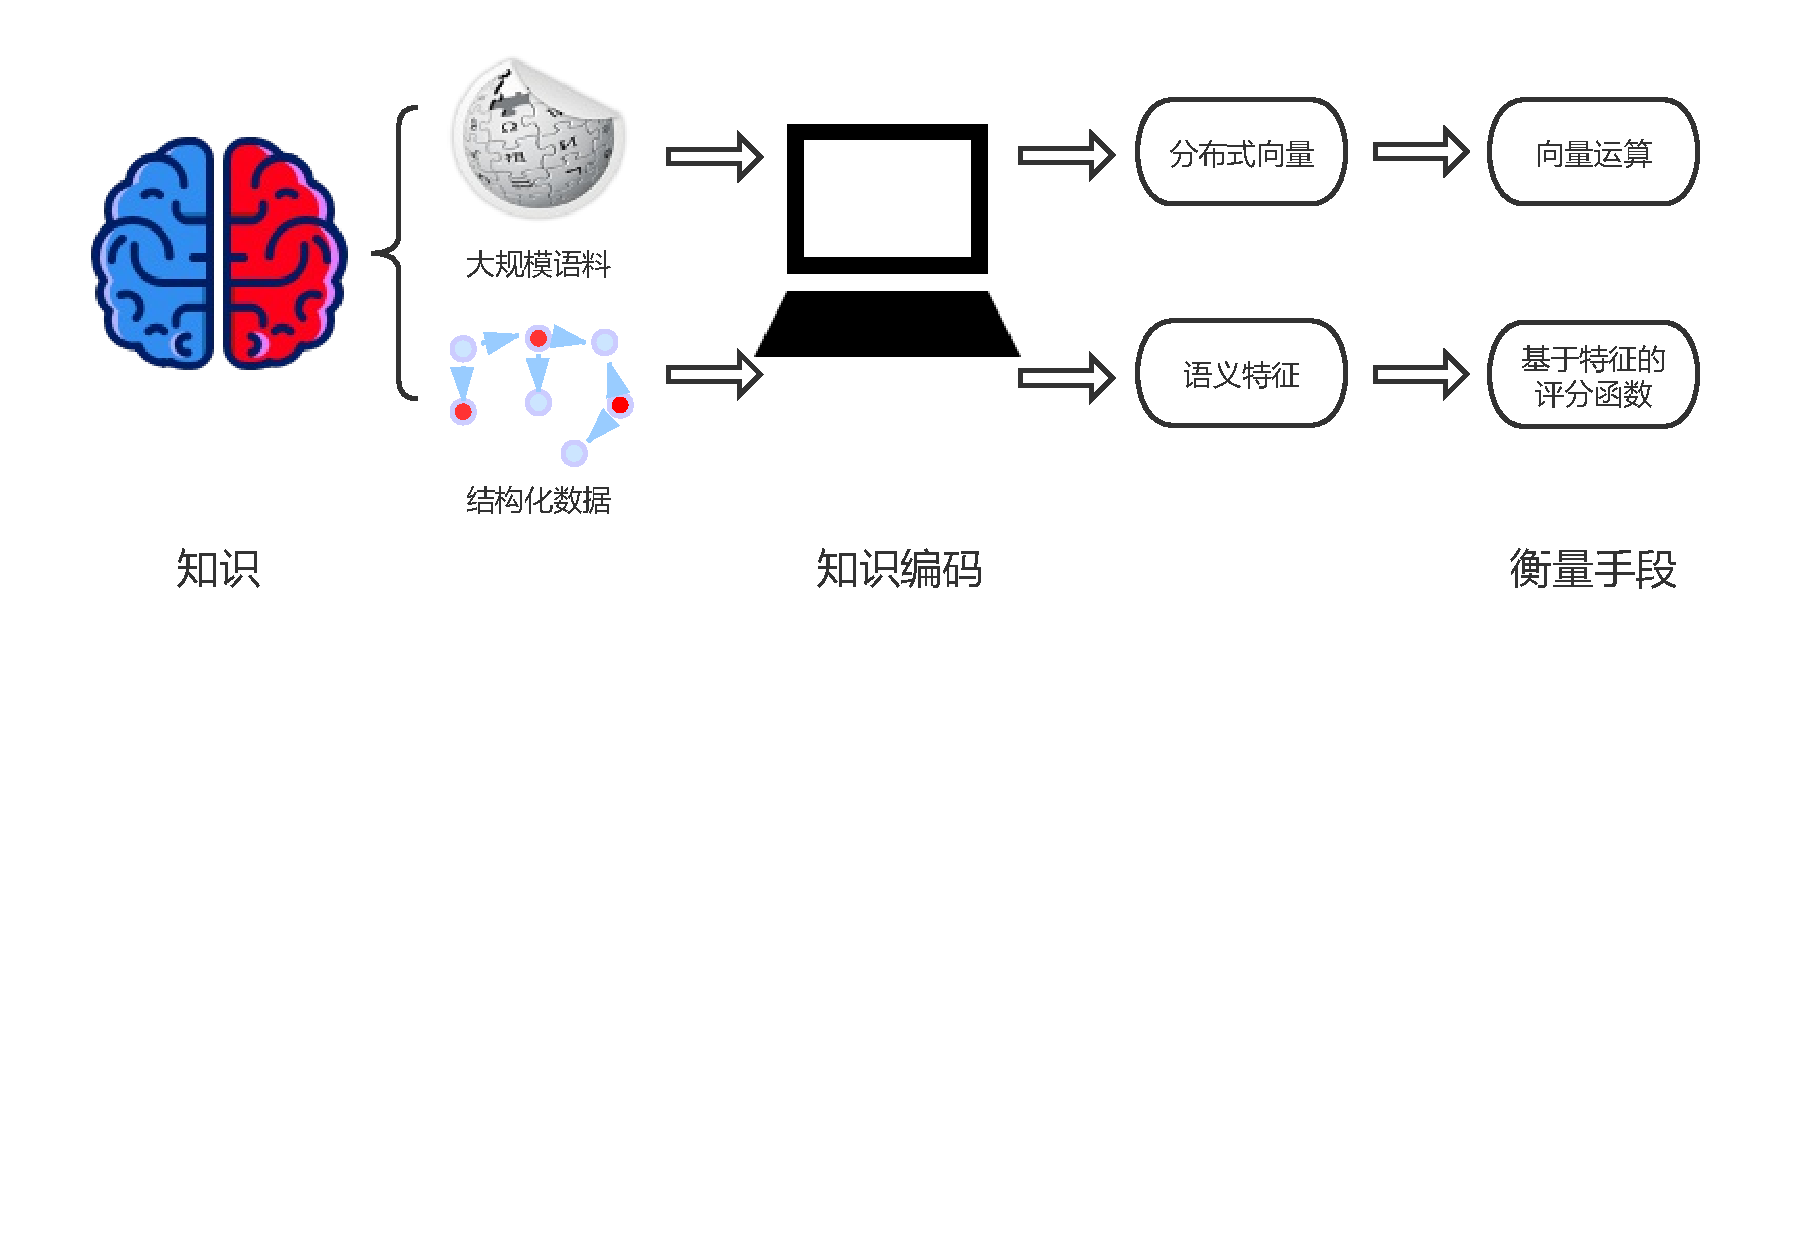
\includegraphics[width=1\textwidth]{chap1-1.pdf}}
    \smallcaption{语义关联度度量简单过程}
    \label{chap1-1}
\end{figure}

对于语义关联度度量,人类会结合自身的认知、经验等来主观并直接地判断两个词语背后包含的知识、意义等之间的相关程度。但是对于计算机来说,如图~\ref{chap1-1},这显得没有那么容易,面临着以下问题:1)知识编码:包含在比较对象中的先验知识无法被简单地转化为数值,无法直接地作为计算机系统的输入;2)衡量手段:当我们可以编码两组对象背后隐含的知识并输入到计算机系统时,针对不同的知识编码方式,采用何种衡量手段来评估语义关联度度量效果也是一个值得研究的问题。

知识的编码往往依赖于知识的存储形式。如表~\ref{knowledge-base}所示,在过去的十几年里,研究者们主要利用以下几种知识存储形式来挖掘词语的意义或语义内容:1)自然语言大规模语料:互联网中存储着丰富的由专业人才构建的高质量自然语言文本,如新闻语料,维基百科\footnote{https://www.wikipedia.org/}等,这些语料中词语的共现信息、词语的上下文信息等都反映了词语的语义内容,因此大规模规范化语料是研究者常利用的一种知识存储形式。2)结构化的知识库:主要包含本体库(Ontology),知识图谱(Knowledge Graph,KG)等,这里作简要介绍:
%
i)在计算机科学与信息科学领域,本体是指一种“形式化的,对于共享概念体系的明确而又详细的说明”~\cite{ka/GRUBER1993199},这是一种直观的形式化的存储形式,反映了领域内知识的层次结构,更加适合在计算机系统中使用,常用的本体库有OWL\footnote{https://www.w3.org/TR/owl-features/}等;
%
ii)大规模语料中的语义信息往往以非结构化或者半结构化的形式存储,为了直观的描述和存储知识,研究者们结合机器抽取和人为标注的方式建立高质量知识图谱,其以三元组(triple)的形式,如WordNet\footnote{https://wordnet.princeton.edu/}、DBpedia\footnote{https://wiki.DBpedia.org/}等,存储着多种多样的实体以及它们之间的关系。通过这样的形式,将知识转化为图结构,方便了后续知识推理、信息检索、语义挖掘等任务的进行。

\begin{table}[!ht]
    \center
    \smallcaption{常用的知识存储形式}
    \vspace{5pt}
    \begin{tabular}{|c|c|c|c|l}
        \cline{1-4}
            & 存储结构 & 主要存储形式 & 实例 & \\ \cline{1-4}
        结构化知识库 & 本体库、知识图谱 & 三元组、图结构 & OWL、WordNet、DBpedia & \\ \cline{1-4}
        大规模语料 & 文本 & 自然语言 & 维基百科 & \\ \cline{1-4}
    \end{tabular}
    \label{knowledge-base}
\end{table}

针对这些知识存储形式,研究者们从下面几个方面入手挖掘知识库中包含的语义信息,由此来完成语义关联度度量:
%
1)基于词法信息的度量方法:研究者们利用WordNet~\cite{acl/Pucher07, tkde/ZhuI17}和Wikitionary~\cite{aaai/ZeschMG08}等知识库来衡量词语间的关联度。他们通过计算知识库中实体之间的路径距离来反映词语间的关联度,距离越近两个词语之间的关联度越高。这种方法在语义相似度衡量任务上表现要优于关联度度量,较好地反映了词语在词法空间或者词语层次结构上的距离,但是由于本体库本身仅仅存储了一些人为构建的词语间层次种属关系,这种方法自然也就无法考虑到词语在语义空间上的信息。
%
2)基于共现原则的度量方法:这种方法认为共同出现在一个句子或窗口中的两个词之间是相关的。大规模自然语言文本中包含着丰富的共现语义信息,为了更全面准确地衡量词语间语义关系,研究者们或从文本中抽取词语之间的关系~\cite{aaai/Milne08},或利用语义分析学习词向量~\cite{ijcai/GabrilovichM07, corr/Mikolov13, emnlp/PenningtonSM14},并且比基于本体库的度量方法取得了更好的效果。但是对于同义词来说,他们几乎不会同时出现在一个句子中,而且共同出现的单词之间也会发生偶发性的不相关现象。
%
3)基于关联网络的方法~\cite{aaai/ZhangZH15, aaai/GongXH18}:为了改善基于共现原则的方法中遇到的问题,这种方法考虑了单词背后的关联实体对关联度度量结果的影响。关联网络最早起源于心理学实验,研究者认为给定一个词,第一个出现在受试者脑海中的词是与给定词最相关的。基于这样的假设,研究者们通过建立关联网络来连接词语与Wikipedia中的实体,由此来丰富词语的语义信息。在建立好的关联网络中,以往的研究中采用大量的启发式评分函数来计算实体之间的语义关联度,再利用此计算结果优化词语间的关联度计算。这种方法虽然在基于大规模语料的统计分析方法基础上,提升了实验性能,但是还面临着一些不足:a)固定的基于规则的启发函数缺乏扩展性和灵活性;b) 对于词语背后的实体关联度比较,这种方法基于规则地从Wikipedia中抽取大量的实体共现信息,实体属性信息以及实体之间的链接信息等,这需要大量复杂的文本预处理。

如上文所述,结构化的知识库中包含着由机器抽取和人为标注构成的高质量信息,本文通过建立词语与知识库实体之间的关联来规避对大规模语料的预处理,其中由词语、知识库实体所构成的网络,我们称之为知识关联网络(Knowledge Association Network,KAN)。对于知识关联网络中的知识库实体,本文通过网络嵌入的方法来学习其分布式向量表示。这种低维的表示可以将实体的多种不同语义信息映射到同一向量空间,然后通过简单高效的向量运算得到实体之间的关联程度。


\section{研究内容}
世界上的各种事物往往都存在各种各样的联系,对于某一种具象事物,其背后往往有多种抽象概念与之对应。图\ref{chap1-2}反映了词语和相关联的实体所构成的网络结构。在这种结构中存在三种关系:
%
1)词语与词语的关系:是指对于给定的一段文本和一个固定大小的窗口,在同一个窗口内出现的词语之间具有联系,这反映了词语与词语的共现关系;
2)实体与实体的关系:词语背后的关联实体作为一种语义补充,在知识库在中表征为有向图,反映了各种实体之间的种属层次关系;
3)词语与实体的关系:对于一个词语,其和不同实体之间的关联程度也是不同的。
%
当利用实体之间的关系来丰富词语的语义信息,并由此来更好地计算词语间的语义关联度时,需要综合考虑这三种关系对结果的影响。面临的第一个问题是如何构建知识关联网络;第二个问题是对于不同的网络形式和规模,如何计算词语间语义关联度。

\begin{figure}
    \centerline{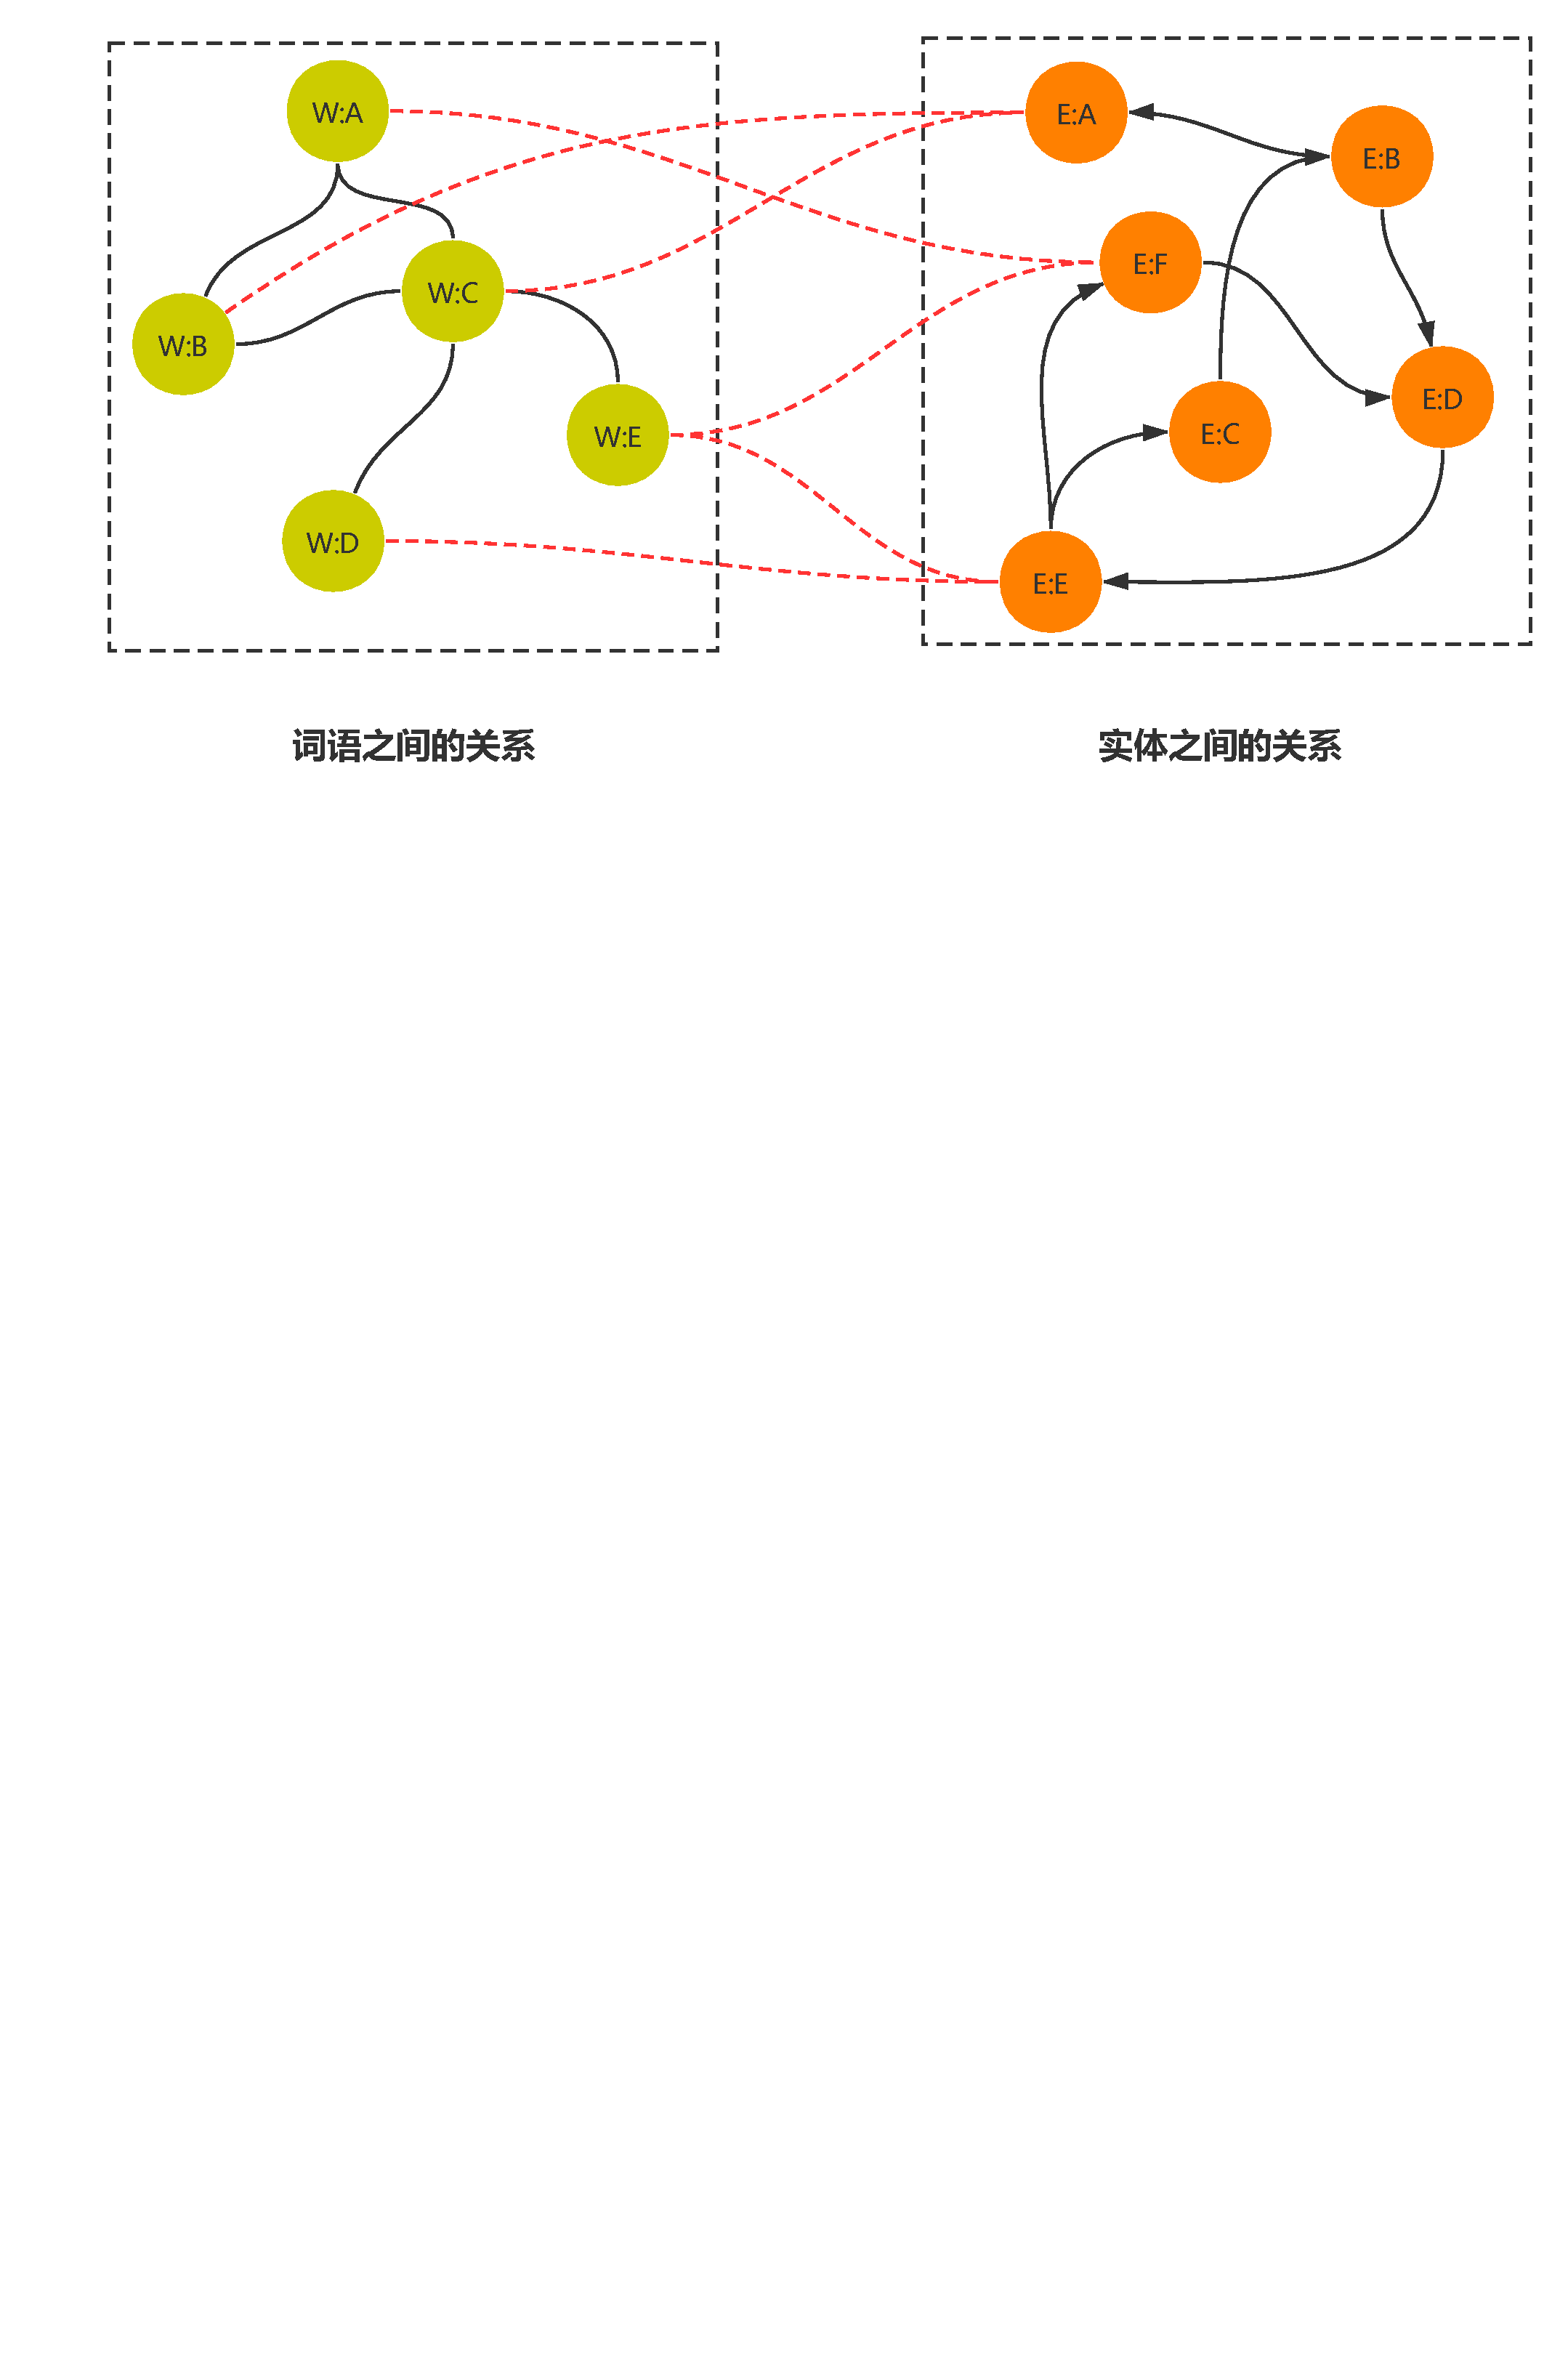
\includegraphics[width=0.8\textwidth]{chap1-2.pdf}}
    \smallcaption{词语和与其相关的知识库实体构成的知识关联网络}
    \label{chap1-2}
\end{figure}

针对第一个问题,即如何构建知识关联网络?其关键是如何建立词语与实体之间的对应关系。对于不同的知识库,建立词语与实体之间关联的方式不同。本文考虑了两种知识库来建立知识关联网络:
1)WordNet作为一种英文词法关系库,其按照单词之间的语义内容和词法关系,将大量英文单词划分为一组组同义词集(synsets),其中包含175979个同义词集和155327个词语,每个同义词集集代表了一个唯一的概念。每个词语与同义词集之间的对应关系也被人为严格准确的标注好并保存在其中,这使得词语与同义词集之间的对应关系可以通过词语字面值匹配被查询到;
2)DBpedia是从维基百科中构建得来的高质量知识图谱,其中每个实体对应于一个维基页面描述的对象。至2016年10月,DBpedia中包含了约600万实体和13亿条RDF三元组\footnote{https://blog.dbpedia.org/2016/10/19/yeah-we-did-it-again-new-2016-04-dbpedia-release/} 。但是DBpedia中没有直接存储词语与实体之间的对应关系,文本首先建立词语与维基页面之间的关系,然后利用实体与维基页面之间的一一对应关系对应到DBpedia中的实体。

第二个问题是在知识关联网络驱动下如何计算语义关联度。本文考虑知识关联网络中包含的三种关系,利用实体层的语义信息来加强词语间的语义关联度度量,而词语与实体之间的关系起到连接词语层和实体层的作用。对于词语层之间的语义关联度度量,本文保留了传统关联网络中的方法,利用词向量~\cite{corr/Mikolov13, emnlp/PenningtonSM14}模型将大规模语料中词语之间的共现关系表示为分布式向量,由此来获得其语义特征。而对于实体层的语义关联度度量,本文分别针对两种不同方式构建的知识关联网络,采用了不同的方法来学习网络实体表示:
\begin{enumerate}
    \item 基于WordNet的知识关联网络驱动的语义关联度计算:WordNet中的实体(同义词集)关系表现为有向图的形式,传统的图注意力网络(Graph Attention Network, GAT)\cite{iclr/VelickovicCCRLB18}多用在有监督或半监督的节点分类任务上,本文提出采用无监督模式的图注意力机制来学习WordNet中实体的分布式向量表示。基于标准测评数据集的实验结果表明,无监督自注意力机制的网络嵌入模型可以更好地学习到实体的向量表示。此外,通过结合WordNet词法向量与文本语料上训练得到的词向量,可以更好的提升模型效果。
    \item 基于DBpedia的知识关联网络驱动的语义关联度计算:DBpedia中的实体数量远超过WordNet中的数量,无监督注意力模型随之变得难以训练。本文将DBpedia中实体的语义信息分为属性空间和拓扑空间,并提出了一种灵活的具有表达力的模型来学习知识图谱中的实体表征。对于实体的属性空间,本文通过最小化正例实体属性对间隔,最大化负例实体属性对间隔的方法来学习其向量表示;而对于实体的拓扑空间,本文首先通过随机游走生成采样序列,然后利用Skip-Gram\cite{corr/Mikolov13}模型去学习实体的向量表示。实验结果证明,此模型进一步提高了语义关联度计算的评测效果。
\end{enumerate}

\noindent 综上所述,本文的贡献有以下几点:
\begin{enumerate}
    \item 本文基于WordNet、DBpedia知识库去构建了知识关联网络,同时考虑了词语与词语、词语与实体以及实体与实体之间的关系对语义关联度度量的影响。
    \item 在知识关联网络的实体层,针对不同的网络结构,本文提出了不同的网络嵌入模型。在基于WordNet构建的网络中,本文将图注意力机制应用到无监督表示学习中;在基于DBpedia构建的网络中,本文同时考虑了实体属性空间与拓扑空间的语义信息。这些分布式向量表示方法在扩展性与灵活性上要明显优于传统模型中人为设计的启发式比较函数。
    \item 基于标准语义关联度度量评测数据集的实验证明,本文的模型要优于几种对比模型,取得了更好的效果。
\end{enumerate}

\section{研究现状}
词语语义关联度计算在生物医学、自然语言处理等应用中扮演者十分基础且重要的角色,其目的是衡量两个词语在语义空间上的距离。本节简要介绍了以往研究者如何利用不同知识表现形式来刻画词语在语义空间上的信息。
%
此外词语背后的语义信息多表现为图的形式,如何更好的将图中信息嵌入到向量空间也是影响关联度度量的关键因素,此外,各种图嵌入模型也在推荐系统,自然语言处理等方面都有重要的应用,本节也将简要介绍了几种常用的图嵌入模型及其应用场景。

\subsection{语义关联度计算的研究现状}
本小节针对不同的知识存储形式,从下面几个方面介绍历史研究者们如何挖掘知识库中包含的语义,如何完成语义关联度度量:

\textbf{基于词法信息的度量方法:}
这种方法基于WordNet和Wikitionary等单词词法库来衡量词语间的语义关联度。WordNet作为一种英文词法关系库,其按照单词之间的语义内容和词法关系,将大量英文单词划分为一组组同义词集。Wikitionary\cite{aaai/ZeschMG08}作为一个人工构造的高质量词法库被提出,旨在为大量的的AI应用提供基础服务。对于一对词语,最早的研究者们\cite{its/Rada89, Leacock98, wu1994verb, tkde/LiBM03}在词法树中找到多条路径连接这两个词,其中最短的一条路径反映了两个词语之间的关联程度。还有一些研究者们,利用WordNet中的同义词集合对应的信息内容(Information Content, IC)值来衡量词语间关联度\cite{ijcai/Resnik95, RCLIC/Jiang97, icml/Lin98},其中IC值被定义为$-log p(c)$,$p(c)$被定义为概念$c$出现在语料库中的频率。由此可见越是具体的概念,比如说“actor”其IC值越高,越是抽象的概念,如“person”其IC值越低。但是这种方法多用来建模词语间的层次关系,在语义相似度方面表现较好,但是对于涉及多种语义关系的关联度度量,这种方法表现不太好。

\textbf{基于共现原则的度量方法:}
为了更好地考虑词语的语义关系,研究者们提出基于词语共现关系来计算语义关联度的方法。即认为在语料文本中,两个词如果共同出现在一个句子或者一个窗口中,则这两个词是相关联的。最初的模型WikiRelate!~\cite{aaai/StrubeP06}利用维基页面中包含的文章类别(Categories)信息来衡量词语间的语义关联度。显式语义分析(Explicit Semantic Analysis,ESA)~\cite{ijcai/GabrilovichM07}首先将维基百科中一篇文章的语义信息表示为高维向量空间,然后通过向量空间的运算来衡量词语间的语义关联度。但是WikiRealted!和ESA仅仅考虑了文本中词语的统计信息,忽略了维基百科中文章之间的链接信息。接下来提出的WLM~\cite{aaai/Milne08}模型利用词语与维基页面中锚文本之间的匹配关系,建立起词语与文章的关系,由此利用文章之间的链接信息提升了词语间语来义关联度度量效果。随后提出的WikiWalk~\cite{textgraphs/YehRMAS09}模型则扩展了WLM模型,进一步考虑维基百科中的页面主体、信息框(infobox)和类别区域中的外链信息建立起文章之间的连接图,然后利用随机游走算法~\cite{emnlp/HughesR07}学习到图中每个节点的向量分布,最后通过向量之间的余弦距离来衡量词语间关联度。SSA\cite{aaai/HassanM11}则利用维基百科中词语上下文中的实体信息为词语构建语义画像,然后通过基于规则的方法计算词语间关联度;Word2Vec\cite{corr/Mikolov13}利用词语之间的共现信息来将词语表征在向量空间,由此来计算语义关联度。

但是上述模型无法有效地建模词语的多种含义,SaSA\cite{aaai/WuG15}利用维基百科词语上下文包含的不同实体为词语分配不同意义,在词义层面学习词语向量表示,解决了Word2Vec中无法表征词语多义性的缺点。而Iacobacci等提出的SensEmbed~\cite{acl/IacobacciPN15}则利用外部知识库BabelNet\footnote{http://babelnet.org}来标注维基语料中词语的不同含义,然后利用Word2Vec~\cite{corr/Mikolov13}模型来学习不同词义的分布式表示。此外,Giuseppe提出的REWOrd模型利用来知识图谱DBpedia和SPARQL查询语言建立起词语与知识图谱之间的联系,由此考虑词语背后的多种含义,然后利用DBpedia中的谓词统计信息来衡量词语之间的语义关联度。

基于共现原则的度量方法有效地考虑词语之间的多种关系,取得了很好的效果。但是对于一些同义词来说,他们几乎不会同时出现在一个句子中,而且共同出现的单词之间也会发生偶发性的不相关现象。接下来要介绍的基于关联网络的度量方法在基于共现方法的基础上利用了词语背后相关的实体中包含的语义信息,有效地提升了度量效果。

\textbf{基于关联网络的度量方法:}
为了改善基于共现原则的方法中遇到的问题,这种方法考虑了单词背后的关联实体对关联度度量结果的影响。关联网络最早起源于心理学实验,研究者认为给定一个词,第一个出现在受试者脑海中的词是与给定词最相关的。基于这样的假设,Keyang~\cite{aaai/ZhangZH15}等人扩大词汇覆盖范围,并通过构造一个词语和概念的关联网络来克服稀疏性,将自由联想(Free Association)规范中的信号和从维基百科的丰富结构中提取的五种类型的共现相结合,这种方法在词语和短文本关联度量中取得不错的效果。Xiaolong\cite{aaai/GongXH18}等人随后提出层次关联网络(Hierarchical Association Network ,HAN)的结构去捕捉词语和Wikipedia实体概念之间的复杂关系,并针对每种关系采用合适的度量方法。通过这种方法,他们取得更好的度量效果。但是,在实体关系比较的过程中,这种模型通过人工设计的特征和固定的统计评分函数去计算实体之间的语义关系。此外,为了得到实体的语义信息,这种方法需要对Wikipedia进行大量的复杂预处理。

文本提出的知识关联网络驱动的语义计算,利用结构化知识库去丰富词语层语义信息,避免了对大规模语料的预处理。同时,本文通过分布式向量表征来表示实体的语义空间,有效地改善了传统手工特征抽取和固定评分函数的不足,取得了不错的度量效果。

\subsection{图嵌入的研究现状}
图作为一种更加普适的结构,反映了各种事物之间的联系,自然界万物之间的关系可以构成一张大图。如何更好地表示的图中的信息成为了各路研究者前仆后继的目标。其中网络嵌入是指根据网络中节点或边所处的网络结构和属性信息,通过一系列技术手段将网络节点或边的各种信息表示在低维向量空间,从而方便后续节点聚类~\cite{aaai/NieZL17}、节点分类~\cite{aaai/WangCWP0Y17}、链接预测~\cite{www/WeiXCY17}以及图分类~\cite{nips/DefferrardBV16}等任务的进行。这其中包含有任务驱动的有监督图表示和无监督图表示。Hongyun Cai~\cite{tkde/CaiZC18}对图嵌入的完整发展和研究现状做了详细阐述,而本文将从以下几个方面简要介绍无监督图嵌入模型的发展过程。

\textbf{基于矩阵分解的图嵌入模型:}
基于矩阵分解的图嵌入模型主要针对图的矩阵表示,通过矩阵分解的技术来将图的结构信息嵌入到低维向量空间。这种方法是最早被研究者关注的图嵌入方法,主要包含两种矩阵分解的方法,分别是基于图拉普拉斯特征映射(Graph Laplacian Eigenmaps)和图邻近矩阵(Proximity Matrix)分解的方法。拉普拉斯特征映射在尽量保留原数据间成对节点相似性的情况下,将处于流形上的数据映射到低维表示~\cite{nips/HofmannB94, nips/HeN03, mm/CaiHH07};图邻近矩阵是一个比邻接矩阵更宽泛的概念,可以反映图节点之间的高阶连接信息,在基于图邻近矩阵的方法中,研究者们直接利用矩阵分解的手段来对邻近矩阵降维得到节点的向量表示\cite{NM/Golub70, nips/HofmannB94}。但是由于矩阵分解本身的计算复杂性,这种方法无法扩展到大图上。

\textbf{基于随机游走的图嵌入模型:}
随机游走作为一种图中常用的采样策略可以有效地捕捉图中节点的结构信息。为了解决基于矩阵分解的图嵌入模型中遇到的问题,这种方法首先通过随机游走策略来生成图中节点的采样序列,然后采用神经网络模型SkipGram\cite{corr/Mikolov13}中的思想来学习节点向量表示。其中SkipGram模型作为一种神经语言模型,最早被应用于自然语言处理领域,此模型通过最大化词语和其邻居节点的共现概率来学习词向量表征。类似的,在图嵌入中采样得到的序列可以被看作一个“句子”,节点和边可以被视为“单词”,通过这种方式可以学习到网络中节点和边的表示。

DeepWalk~\cite{kdd/Perozzi14}最先采用SkipGram模型来训练截断随机游走策略生成的序列,所谓截断随机游走是指均匀随机采样最后一次所在节点的邻居,直到达到设定的最大采样长度。受DeepWalk的启发,后续又有大量的工作针对不同的应用修改随机游走的采样策略~\cite{ijcnn/JinLLZZW16, kdd/GroverL16, icml/YangCS16}。其中应用比较广泛的是node2vec~\cite{kdd/GroverL16},这个模型设计的偏置随机游走通过两个参数可控地调节随机游走过程中的游走方向,结合了图的深度优先遍历与广度优先遍历,取得不错的效果。然而这些模型往往针对的是同构图,在异构图嵌入方面,metapath2vec~\cite{kdd/DongCS17}提出了基于定义好的元路径的随机游走策略,并利用SkipGram来学习节点向量表示,弥补了传统游走策略在异构图上的不足。此外,除去SkipGram模型之外,还有一些模型尝试了LSTM~\cite{neco/HochreiterS97},GRU~\cite{ssst/ChoMBB14}等模型来学习节点或整个序列的表示\cite{aaai/LiuZZZCWY17, www/LiMGM17},并取得了不错的效果。

\textbf{基于神经网络的图嵌入模型:}
这种方法又称为图神经网络(Graph Neural Network,GNN),主要采用卷积神经网络~\cite{MP/Yann},注意力机制~\cite{corr/VaswaniSPUJGKP17}以及自编码器~\cite{icml/VincentLBM08}等深度网络模型来学习网络节点和边的表示。Zonghan Wu~\cite{corr/Zonghan19}等人对GNN的发展和应用场景做了全面详尽的总结。其中适用于无监督图嵌入的模型主要有图自编码器和基于负采样的图嵌入模型。其中在基于自编码器的图嵌入模型~\cite{corr/KipfW16a, ijcai/PanHLJYZ18}中,编码层将图中节点和边转化为低维向量表示,然后解码器通过这些向量表示重构图模型,这种方式可以在中间层学习得到节点和边的向量表示。另一种基于负采样策略的图嵌入模型~\cite{nips/HamiltonYL17}首先通过采样得到多组不相关节点作为负例,图中已经存在的直接相连的节点作为正例,通过最大化负例样本之间的距离,最小化正例样本之间的距离这样的方式来完成图嵌入。

\section{文章组织结构}
本文的整体结构组织如下:

第一章:绪论:

在这部分,本文主要从整体上阐述了知识关联网络驱动的语义关联度的的研究背景和选题意义,同时对本文的的的研究内容和主要解决的问题做了大致阐述,最后简要介绍了词语间语义关联度计算以及无监督图模型的研究现状和主要面临的问题。

第二章:知识关联网络的构建:

本章开头以一个简单的例子解释语义关联度与语义相似度的概念,并分别给出定义,随后针对知识关联网络构建过程中遇到的概念做了简单阐述。最后从整体上介绍如何统筹知识关联网络中边的三种类型来计算最后的关联度值,并给出算法流程。

第三章:基于wordnet构建的知识关联网络驱动的语义关联度计算:

这部分首先对WordNet进行了简要的介绍,并抽取出WordNet中的多种实体关系来构建知识关联网络。之后,对于实体层的网络结构,本文采用更具表达能力图注意力网络机制来学词实体的分布式向量表示,由此利用词语在WordNet中关联实体的语义信息来丰富词语间的语义关联度度量。


第四章:基于DBPedia构建的知识关联网络驱动的语义关联度计算:

这部分首先对DBpedia进行了简要的介绍,然后综合考虑文本外链与文章对词语的影响来计算词语与实体的关联度,由此构建基于DBpedia的知识关联网络。最后提出的实体嵌入方法,综合学习了实体周围的属性信息及其网络结构的拓扑信息,由此在向量空间丰富词语的语义信息。

第五章:实验设计与结果分析:

实验部分基于传统评测数据,给出了多种对比模型在语义关联度任务上的表现。对于基于WordNet构建的知识关联网络,本文对比了多种网络嵌入模型的表现,验证了基于自注意力机制的无监督网络嵌入模型的效果;而对于基于DBpedia构建的知识关联网络,本文对比了实体层实体属性空间与拓扑空间语义信息对最后关联度度量结果的影响。最后通过与传统基准模型的对比,验证了本文提出的模型的效果。


第六章:总结与展望:

最后,这部分对全文知识关联网络驱动的语义关联度计算做出总结,归纳研究过程中遇到的问题,分析语义关联度计算中仍存在的挑战,并对未来的工作计划做进一步展望。
